% !TEX root = ../thesis.tex
\chapter{Approach}
\label{ch:approach}
% **************************** Define Graphics Path **************************
\ifpdf
\graphicspath{{Chapter3/Figs/Raster/}{Chapter3/Figs/PDF/}{Chapter3/Figs/}}
\else
\graphicspath{{Chapter3/Figs/Vector/}{Chapter3/Figs/}}
\fi

\section{Introduction}
\label{sec:approachIntro}
Despite the importance of crowd monitoring in mass gathering events, the literature review in the previous chapter has identified several gaps in the research, especially in crowd modelling. Most state-of-art crowd monitoring techniques do not incorporate a typology to identify and distinguish different types of crowd. In other words, they lack the capability to make distinction of different crowd types that can occur in a mass gathering event. To address this issue, our proposed approach employs one of the most famous existing works on definition of crowd types in emergency management - the \citet{Berlonghi1995}'s model. Our approach also automates the classification of crowd type by considering the emotional conditions of the crowd. Those novelty attempts are integrated into a complete framework for real-time crowd monitoring, which will be discussed in detail in this chapter.

This chapter is structured as follow. Firstly, the overview of our proposed crowd monitoring framework will be introduced. Then each component in the framework will be discussed in the following sections. The chapter ends with the conclusion which will give a summarised look at the framework.

\section{An Overview of the Crowd Monitoring Framework}

The literature review in Chapter \ref{ch:litReview} has summarised that most of the state-of-art crowd monitoring approaches are focusing on using computer vision to automate the analysis of CCTV system. The literature review has revealed several limitations of the computer vision technique, such as the effect of obstacles and low lighting condition. With the rapid development of mobile computing and the increasing popularity of mobile devices, mobile sensing seems to be a more potential technique to collect contextual data for crowd monitoring, for example GPS receivers and accelerometers. Context data refers to all the knowledge that is related to a crowd. Context data can be at raw level such as the acceleration and rotational forces generated by accelerometer built in a participant's mobile phone, or at high level such as the current activity that the user is performing using activity recognition techniques.

Apart from the ``hard sensors'' where physical sensors are used, the literature review also highlights that another type of information source known as the ``soft sensor'' can be used to monitor the crowd and detect the occurrence of stampede in a crowd which is the social media \citep{Ramesh2014}. The use of social media analysis for crowd monitoring has been introduced in a related work by \citet{DelirHaghighi2013}. It has the great advantage of feasibility as it only relies on the software and no additional hardware is required to be installed. Despite this strength, our literature review shows that very limited works have been done to utilize social media to support crowd monitoring in emergency management.

Secondly, another finding from the literature review is that the actual behaviour of a crowd depends largely on the emotions of the participants \citep{Kornblum2011, jasper2011emotions}. For that reason, it is essential for a crowd monitoring approach to consider the influence of emotions in the crowd. Although human emotion is an abstract concept and very difficult to measure with ``hard sensors'', it is possible to capture the emotion of a person from the verbal expressions, such as text \citep{alm2005emotions} or speech \citep{sobin1999emotion}. This is where social media further proves its advantage over the ``hard sensors''. By applying analysis on the social media, we can capture the emotions in a crowd, thus enabling the inference of the crowd's condition. For that reason, this project will propose a crowd monitoring framework that employs the emotion analysis of social media to support emergency management in mass gatherings by determining the current type of the crowd. 

Finally, the literature review also reveals another gap in the research that is the limitation of the crowd modelling employed in crowd monitoring approaches. Most existing crowd monitoring techniques do not base on any crowd model which can distinguish between different crowd types and identify the exact crowd type that is happening without the interpretation of human. By exploring broader into other disciplines, our literature review points out several notable works on crowd modelling and classification in the police literature and public safely science. Among those works, \citet{Berlonghi1995}'s work stands out as the most commonly adopted model by the emergency management bureaus worldwide. Our proposed crowd monitoring framework is established on the \citet{Berlonghi1995}'s model which consists of eleven different crowd types. Yet, a systematic approach to classify one crowd into those types is challenging because \citet{Berlonghi1995}'s model only describes the crowd types and there is no attribute or method defined in the existing model to make the distinction between them. Therefore, in our approach, we would like to propose a mapping model that connects the emotion model with the crowd model, enabling the fuzzy classification of crowd type by emotions. The reason fuzzy logic is utilized in our approach is because of its capability of representing multiple truths rather than the absolute true or false like in classical logic. It is difficult to divide people in a mass gathering into very distinct classes using rule-based reasoning since crowd types can be overlapping. Fuzzy logic is able to calculate the degree of membership of each crowd type in a particular crowd and represent the real-time and gradual changes in crowd type.

In conclusion, our proposed approach will address the gaps that are identified in the previous chapters by: 
\begin{inparaenum}[i)]
\item incorporating social media as the information source for context data;
\item capturing the emotions of a crowd by analysing the context data from soft sensors;
\item identifying the type of a crowd by applying fuzzy rule based inference to the crowd emotions
\end{inparaenum}. These objectives can be integrated together in a complete process as illustrated by Figure \ref{fig:processOverview}. Social media is firstly probed to get the context data at the raw level. This raw data is then processed in an emotion analysis to extract high level context data, that is the emotional states of the crowd. These emotional states are in turn used as the attributes or features to classify a crowd into a specific type.

\begin{figure}[htb!] 
\centering    
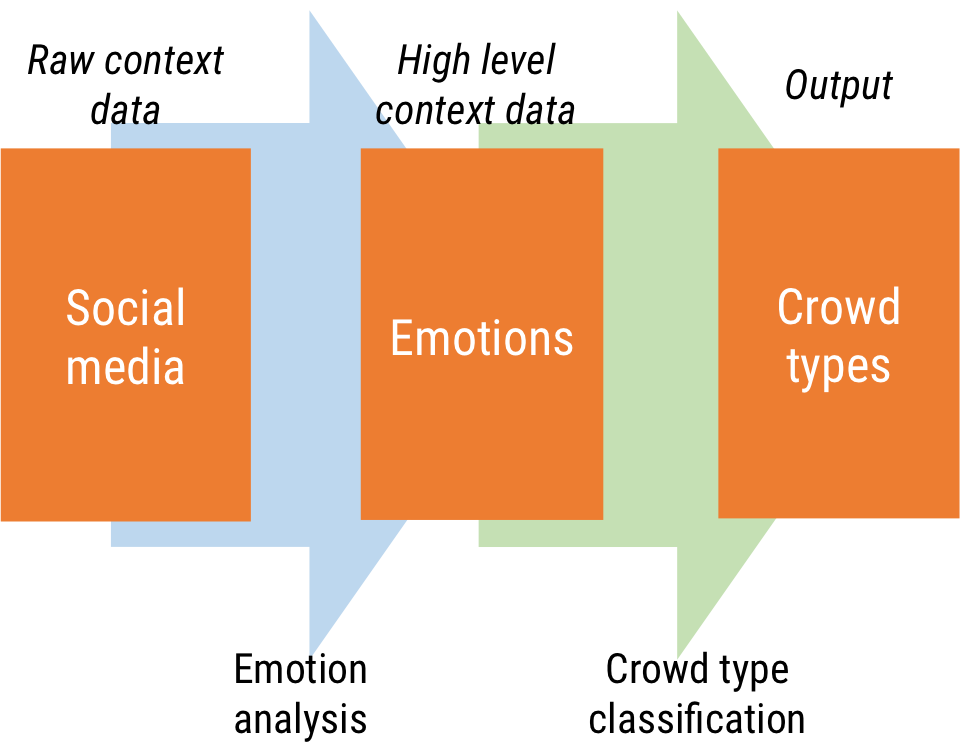
\includegraphics[width=0.5\textwidth]{ProcessOverview}
\caption{A process to identify a crowd type from social media}
\label{fig:processOverview}
\end{figure}

From the functional point of view, the process can be implemented into a framework. Figure \ref{fig:frameworkOverview} shows our framework consisting of following components:
\begin{inparaenum}[i)]
\item Context data;
\item Emotion analysis;
\item Emotion model;
\item Crowd model;
\item Emotion - Crowd type mapping model;
\item Rule based reasoning
\end{inparaenum}. Each component will be discussed further in the sections below.

\begin{figure}[htb!] 
\centering    
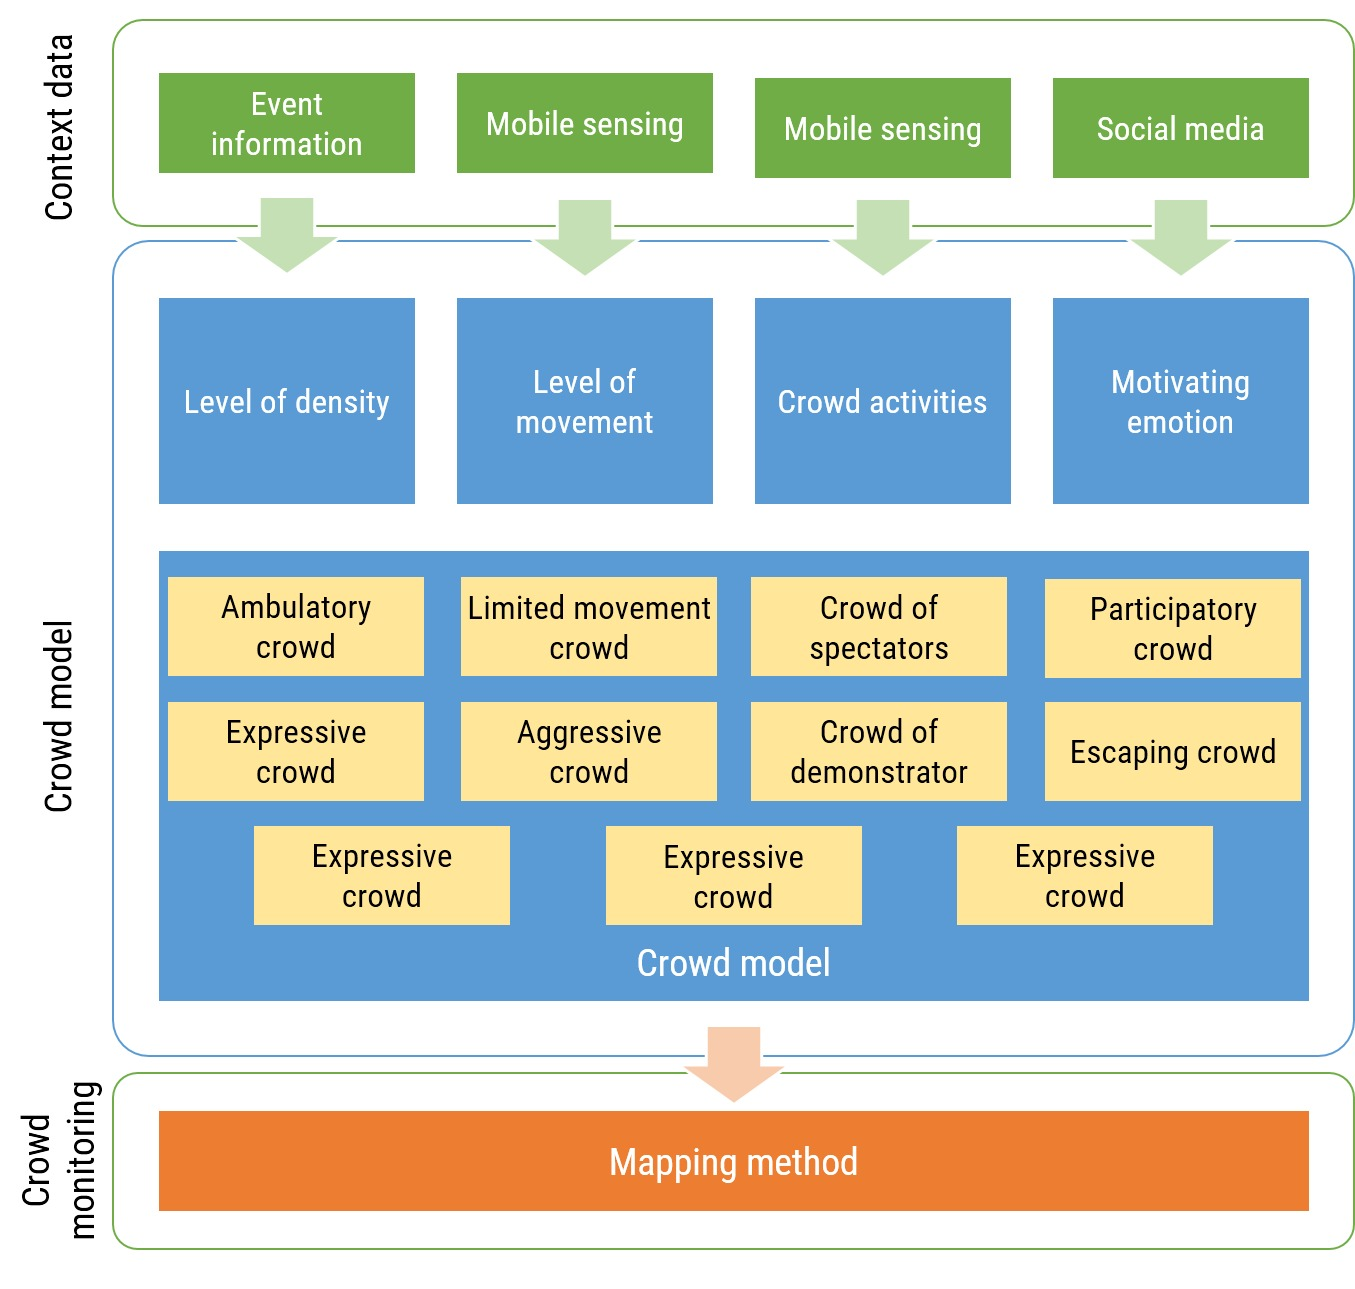
\includegraphics[width=1.0\textwidth]{FrameworkOverview}
\caption{An overview of the crowd monitoring framework using emotion analysis of social media}
\label{fig:frameworkOverview}
\end{figure}

\section{Context Data}
The first component of the framework is the Context Data component. In our proposed framework, contextual data is gathered from the social media as the information source. Social media is the generic term referring to a wide range of Internet based tools that enable a user to create and share information with each other \citep{kaplan2010users}. These tools include social network services such as Facebook and Twitter, blogs, Internet forums and channels which have marked the beginning of Web 2.0. Unlike other traditional media such as newspaper or television, the content on social media is created by the users, or also known as user-generated content \citep{kaplan2010users}. User-generated content can be in various formats such as text, image or video. Because of the fact that the content is being generated by the users themselves, social media is an effective source to obtain the knowledge about the users. In our domain and application of crowd monitoring, the kind of knowledge that is important to capture is the emotional state of the participants in the crowd. 

In our research, we will focus on the use of social media, or Twitter in particular, as the information source for context data, because of the following reasons. Firstly, among social media, Twitter is the most commonly used in researches because of its large volume of users and its public APIs which make the data highly accessible. The user-generated content is mostly text-based and in the form of a short message which has no more than 140 characters called tweet. Because of this length limit, a tweet is usually very simple in term of the meaning and each tweet focuses on expressing the idea of the author on one particular topic. This fact makes the a semantic analysis of tweets more feasible in real-time than other content, for example, a long blog article.

A tweet might also contain information beyond the text. A significant number of tweets are geo-tagged, which means they are attached with the location information when they are posted to Twitter. This location information can be in the form of exact coordinates if the user posts the tweet from a GPS enabled mobile phone. Alternatively, this location might also be a relative location such as point of interests or town if the user checks in or attaches a place with the tweet.

Another useful information that might exist in a tweet is hashtags. Hashtags are created by the users, and usually are put in a tweet to refer to the topic that is mentioned in the tweet \cite{mohammad2014using}. In some mass gathering events such as the Australia Open or music festivals, there are pre-defined hashtags created for these particular events so that a user can put the hashtags into his tweet when mentioning about the events. Similarly to the geo-location, this information can also be used to filter for tweets belonging to a specific event.

Finally, using Twitter as the information source for crowd monitoring has some certain advantages. Firstly, the data can be collected in real-time, enabling the real-time monitoring which is an essential operation in emergency management because of the dynamic nature of a crowd that it can change from a calm type to an aggressive type \citep{Berlonghi1995}. Secondly, it does not require any pre-installed hardware or software on the participants, which increases the feasibility of our proposed framework.

\section{The Emotion Model}

From the literature review, a crowd type can be described as a form of collective behaviour of a group of people in close proximity. The other form of collective behaviour is mass which involves people dispersed in a large area and does not belong to our context of emergency management in mass gathering. Both the Convergence Theory and the Emergent Norm Theory \citep{mcphail1991myth} support the idea that a crowd behaviour is formed by people with a common motivation. In our framework, we emphasize on the emotional factor as the common motivation of the behaviour in the crowd. Different emotions can consequently lead to different crowd behaviours. For example, according to Lofland's typology of spontaneous collective behaviours \citep{Kornblum2011}, a panic exodus from burning theatre is motivated by the fear whereas a race riot is aroused by the anger. Therefore, an emotion model is essential to distinguish different emotions of the people in the crowd.

Human emotion is no doubt complex and confusing \citet{plutchik2001nature}. Therefore, it is difficult even to just list all emotions, not to mention modelling them. However, it is often assumed among theories of emotions that there exists a small set of basic or fundamental emotions, yet there is still little agreement on the number of basic emotions and what emotions are in the list \citep{Ortony1990}. Based upon the theory of evolution of the biological process, \citet{plutchik2001integration} was able to identify eight basic emotions consisting of four pairs of opposite emotions: \textit{anger/fear}, \textit{joy/sadness}, \textit{trust/disgust}, \textit{anticipation/surprise}. Investigating the facial expression of human, \citet{ekman1971constants} suggested there are six basic emotions that can be universally recognised, regardless of the language. The six basic emotions are \textit pit{anger}, \textit{fear}, \textit{happiness}, \textit{sadness}, \textit{surprise} and \textit{disgust} as illustrated in Figure \ref{fig:emotionModel}. Ekman's model has been adopted in many researches regarding human emotions \citep{mohammad2014using, roberts2012empatweet, alm2005emotions}. 

\begin{figure}[htb!]
\centering    
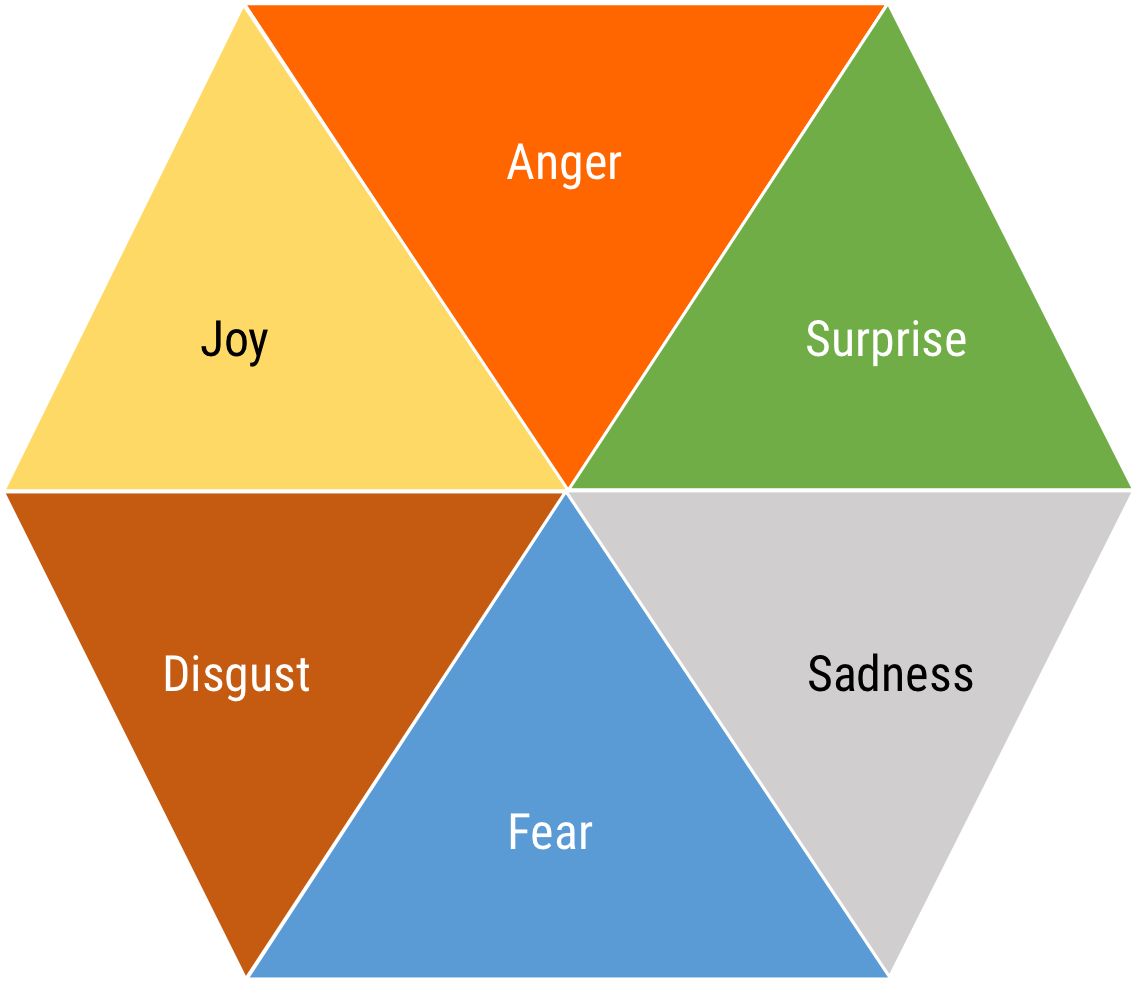
\includegraphics[width=0.75\textwidth]{EkmanModel}
\caption{Ekman's six basic emotions}
\label{fig:emotionModel}
\end{figure}

A recent research by \cite{Jack2014} has pointed out the similarity during the early signal of the facial expression between anger and disgust, as well as surprise and fear. For example, both anger and disgust share a wrinkled nose, while both surprise and fear share raised eyebrows. Based on these findings, they suggest only four basic emotions, as can be seen from Figure \ref{fig:emotionModel}.

In our proposed framework, the basic emotions are employed as the features to classify the crowd type. Because the description of the crowd types, which will be mentioned in more detail in the next section, does not specify any related emotions, it is difficult to identify which emotions associated to a particular crowd type. Using an emotion model with fewer basic emotions, each of which completely differs from the others, effectively addresses this difficulty. Therefore, the four most basic emotions consisting of \textit{anger}, \textit{fear}, \textit{happiness} and \textit{sadness} will be adopted as our emotion model in the proposed framework.

\section{The Emotion Analysis of Social Media}

A recent analysis on the content on Twitter reveals that the users are using Twitter for a variety of purposes, which can be grouped in two main types: updating their statuses or sharing information \citep{java2007we}. Regardless of the content in both cases, a tweet often conveys the author's emotional status \citep{bollen2009modeling}. By capturing the emotion expressed in the text, it is possible to infer the emotional state of the author. In our framework, as can be seen from Figure \ref{fig:processOverview} a tweet can be considered as a raw context data collected from the information source whereas the emotion in the tweet is the high-level context data that is inferred and it will be used in our proposed crowd type classification. This transformation from the raw-level to the high-level context data is performed by the Emotion Analysis component. 

Regarding emotion detection from tweets, there have been several related works such as from \citet{bollen2009modeling}, EmpaTweet by \citet{roberts2012empatweet} and NRC Hashtag Emotion from \citet{mohammad2014using}. The common approach that was employed in these works is the Bag-Of-Words which only considers the occurrence of words while ignoring the grammar and the meaning. Our Emotion Analysis also incorporates the Bag-of-Words approach illustrated in Figure \ref{fig:bagOfWord}.

\begin{figure}[htb!] 
\centering    
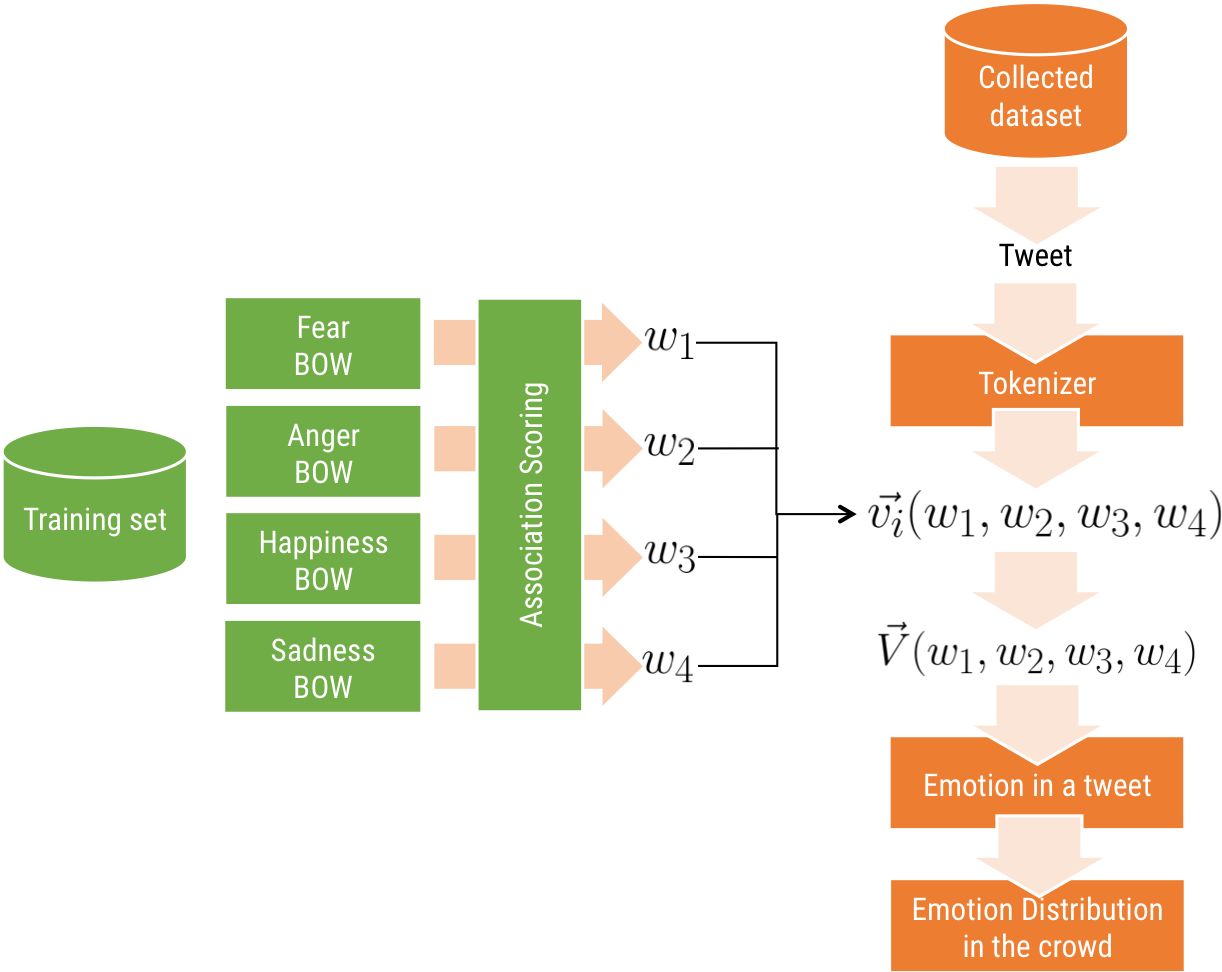
\includegraphics[width=1.0\textwidth]{BagOfWord}
\caption{An overview of the Bag-of-Words approach}
\label{fig:bagOfWord}
\end{figure}

\subsection{The Bag-of-Words Approach}
The Bag-Of-Words approach is based on a simplified representation of a document introduce by \citet{joachims1996probabilistic}. This representation only considers at the frequency of appearance of the words in a document while disregarding the grammar and the order of the words. In our case with Twitter, a document is a single tweet and a word is an uni-gram what builds up the tweet. The process that splits a document into a sequence of words is called tokenizer. In our experiment which will be mentioned in Chapter \ref{ch:eval}, the Stanford NLP Tokenizer \footnote{http://nlp.stanford.edu/software/tokenizer.shtml} is applied to tokenize a tweet into words and also to filter out unwanted text, such as URLs and emoticons. 

\begin{figure}[htb!] 
\centering    
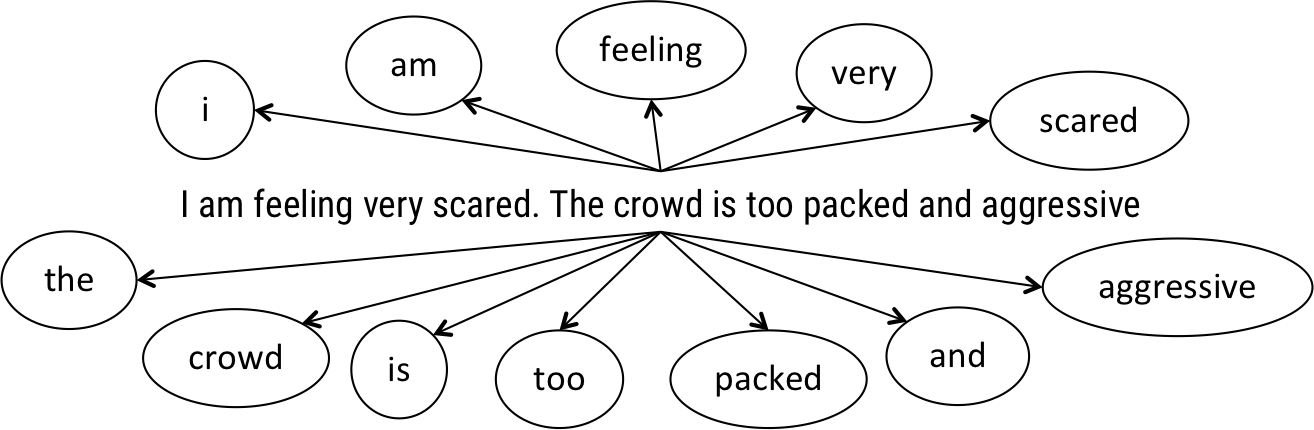
\includegraphics[width=0.5\textwidth]{Tokenizer}
\caption{An example of a tweet tokenized into words}
\label{fig:tokenizer}
\end{figure}

As mentioned earlier, a few related works on emotion analysis also employed the Bag-of-Words approach. \citet{bollen2009modeling} used an extended version of the Profile of Mood States (POMS) with 765 terms from 65 original mood adjectives. These terms were used to match with the words extracted from a tweet, in order to map a tweet with the six POMS moods: \textit{tension}, \textit{depression}, \textit{anger}, \textit{vigour}, \textit{fatique} and \textit{confusion}.

The EmpaTweet by \citet{roberts2012empatweet} collected tweets on 14 selected topics that each topic was expected to evoke a particular emotion in seven emotions: \textit{anger}, \textit{disgust}, \textit{fear}, \textit{joy}, \textit{sadness}, \textit{surprise} and \textit{love}. The collected tweets formed the labelled corpus which was used to train the machine to automatically detect the emotions from Twitter. The classification was performed by a series of SVM classifiers with uni-grams, bi-grams and tri-grams of words as features of a tweet.

The NRC Hashtag Emotion by \citep{mohammad2014using} was another notable work which made a good use of the hashtags as the labelled data. Tweets that were attached with these hashtags: \textit{\#anger}, \textit{\#disgust}, \textit{\#fear}, \textit{\#joy}, \textit{\#sadness} and \textit{\#surprise} and their synonyms were collected. These hashtags were considered to be the label of a tweet, which depicted the emotion in the tweet. The experiment also verified that the self-labelled hashtags were consistent and matched with the annotation by trained judges. The collected tweets constructed the NRC Hashtag Emotion Corpus. Using the corpus, \citet{mohammad2014using} computed the association of each word with Ekman's six emotions which was called the Strength of Association (SoA). This SoA score of a word can take the value from 0 for no association to infinity indicating maximum association to a specific emotion. The collection of words and their SoA were known as the NRC Hashtag Emotion Lexicon, which has been published and available for research purposes \footnote{http://saifmohammad.com/WebPages/lexicons.html}.

Our Bag-of-Words approach performs a similar process. Firstly, a Bag-of-Words for each emotion \textit{anger}, \textit{fear}, \textit{happiness} and \textit{sadness} are constructed from the training set which contains tweet labelled with emotion. The Association Scoring measures the association of a word with anger, fear, happiness and sadness represented by four normalised weights \(w_1\), \(w_2\), \(w_3\) and \(w_4\) respectively. As a result, the emotion model of a word can be represented by a four dimensional vector \(\vec{v_i}(w_1, w_2, w_3, w_4)\) called ``emotional weight vector'', which takes the four weights as the dimensions. Secondly, in the real-time analysis, a tweet is tokenized into words, each of which will have an emotional weight vector. A voting system will then calculate the dominating emotion of a tweet from the emotional weight vectors of its words. Finally, the distribution of each emotion in the sampling data is then calculated to detect the emotions in the crowd. Each component in this process will be discussed in the next section.

\subsection{The Training Set}
The training set, or labelled corpus, is a collection of tweets which are labelled with correct emotions to server as the training data for classifiers. In our research, the NRC Hashtag Emotion Corpus by \citet{mohammad2014using} was chosen as the labelled set because of following advantages. Firstly, both the NRC Hashtag Emotion Corpus as well as the EmpaTweet Corpus were annotated with Ekman's six basic emotions which contain our four basic emotions. Secondly, by collecting tweets with emotional hashtags, the NRC Hashtag Emotion Corpus is more generic and it can be applied to other topics with a higher accuracy compared to the EmpaTweet that is limited to the selected topics.

\subsection{Association Scoring and the Emotional Weight Vector}
As mentioned in the Association Scoring process, the association of a word with a specific emotion must be measured by a normalised weight. This weight represents the correlation of the word with the emotion and it must be comparable with with other words and other emotions. From the related works, it can be noticed that the SoA score proposed in the NRC Hashtag Emotion Lexicon by \citet{mohammad2014using} is effectively suitable for this purpose. The SoA is calculated from the frequency of a word appearing in the tweets tagged with an emotion.

Therefore, in our Emotion Analysis, the SoA score will be employed as the normalised weight indicating the association of a word with an emotion. The emotional status of a word can be modelled by a four dimensional vector with each dimension represents an emotion of the basic emotions: anger, fear, happiness and sadness. This vector is proposed as the ``emotional weight vector'' as in Formula \ref{eq:emotionalWeightVector} below.

\begin{equation}
\label{eq:emotionalWeightVector}
	\vec{v_i}(w_1, w_2, w_3, w_4)
\end{equation}
where \(v_i\) is an ``emotional weight vector'' of a word and \(w_{1,2,3,4}\) are four weights that represent its association with the four emotions: anger, fear, happiness and sadness respectively. For example with the word ``crowded'', the SoA scores are taken from the NRC Hashtag Emotion Lexicon as presented in Table \ref{table:soaOfCrowded}. Four scores for anger, fear and joy (happiness) and sadness are extracted and construct the ``emotional weight vector'' of ``crowded'' as in below Formula \ref{eq:emotionalWeightVectorOfCrowded}.

\begin{equation}
\label{eq:emotionalWeightVectorOfCrowded}
	\vec{v_{crowded}}(0.0630391396873302, 0.853341316895822, 0, 0)
\end{equation}

\begin{table}
\caption{SoA scores of ``crowded'' toward the eight basic emotions (Taken from NRC Hashtag Emotion Lexicon \citep{mohammad2014using})}
\label{table:soaOfCrowded}
\centering
\begin{tabular}{|l|l|}
\hline
\textbf{Emotion} & \textbf{SoA score} \\ \hline \hline
Anger & 0.0630391396873302 \\ \hline
Fear & 0.853341316895822 \\ \hline
Joy & 0 \\ \hline
Sadness & 0 \\ \hline
Trust & 0 \\ \hline
Disgust & 0.201742824294623 \\ \hline
Anticipation & 0 \\ \hline
Surprise & 0 \\ \hline
\end{tabular}
\end{table}

\subsection{The Voting System and the Dominant Emotion}
The emotional status of one word can be modelled by a four dimensional ``emotional weight vector''. A tweet can be considered as a set of words, each of which contributes to the overall emotional status of the tweet. Therefore, the emotional status of a tweet can also be represented by a four dimensional vector that is the summative of the ``emotional weight vectors'' of the elemental words (Formula \ref{eq:summativeWeightVector}).

\begin{equation}
\label{eq:summativeWeightVector}
	\vec{V} = \sum_{i=1}^{n} \vec{v_i}(w_1, w_2, w_3, w_4)
\end{equation}
where \(\vec{V}\) is the ``emotional weight vector'' of the tweet, \(\vec{v_i}\) is a weight vector of word \(i\) and \(n\) is the total number of words in the tweet.

Although a tweet might be associated with all four emotions, one specific emotion is expected to dominate the whole tweet, which is called the dominant emotion. In order to extract the dominating emotion in a tweet, a voting system to interpret the vectors is proposed as follow. An ``emotional weight vector'' \(\vec{v_i}\) can be considered as a vote cast by one word that indicates how strongly the word agrees with each emotion. Similarly, the summative vector \(\vec{V}\) can be interpreted as the overall result of the voting, which illustrates how close the whole tweet is from each emotion. The dominant emotion can then be determined by the highest vote from the voters. In other words, the emotion dimension with the largest magnitude will be selected as the dominant emotion in the tweet.

\subsection{Distribution of Emotions in a Crowd}
As illustrated by Figure \ref{fig:processOverview}, the tweets collected in the first stage of the process provides the context at the raw-level about a crowd in a mass gathering. By performing the emotion analysis, the dominant emotion in each tweet can be extracted. This emotion in fact represents the emotion of an individual in the crowd rather than the crowd as a whole. The relationship between individual emotion and group emotion has been discussed in several researches. \citet{barsade1998group} suggest the top-down approach that the group emotion can arise and felt by individual member, while at the same time, in a bottom-up manner the group emotion can be shaped by the compositional effects of individual emotions. This theory confirms the possibility to represent the crowd emotion as whole from the individuals' emotion.

As people with different emotional states can exist in one crowd, a crowd can have multiple emotion. It can be illustrated by the distribution of the emotions in the crowd. The distribution \(d\) of an emotion \(e_i\) in a crowd at a given time \(t\) can be calculated by below Formula \ref{eq:distributionEmotion}.
\begin{equation}
\label{eq:distributionEmotion}
	\forall e_i \in \{anger, fear, happiness, sadness\}: d(e_i)_t = \frac{n(e_i)_t}{N_t}
\end{equation}
where \(d(e_i)_t\) is the distribution of emotion \(e_i\), \(N_t\) is the total number of data sampled during \(t\) and \(n(e_i)_t\) is the number of data classified with emotion \(e_i\) among \(N_t\).

This distribution \(d(e_i)\) can have any value from 0 to 1, indicating the how strong the emotion \(e_i\) of the crowd is at specific time period \(t\). This calculation is performed repetitively after an interval which enables us to detect the change of emotional state in the crowd. Hence, the value of \(t\) has influence on the sensitivity of the detection and depends on the sampling rate.

\subsection{Labelling the Level of Density of an Emotion}
Although the distribution of an emotion in a crowd is able to show the significance of that emotion compared to others, it is not sufficient to tell whether the level of an emotion is normal or not, especially in term of intensity. Hence, such linguistic labels as low, medium and high are defined to identify different level of intensity of an emotion. The intensity increase with the increasing of the level from low to high. There are certain points in the degree of membership that the intensity of an emotion changes from low level to medium level and from medium level to high level (Figure \ref{fig:levelOfDensity}). These two points are defined as threshold \(t_1\) and \(t_2\) respectively. The conversion from numerical values of the distribution of emotion \(e_i\) to a linguistic label can be performed by following rules.
\begin{equation}
\label{eq:lowDensityEmotion}
d(e_i) \leq t_1(e_i) \Rightarrow label = low
\end{equation}

\begin{equation}
\label{eq:mediumDensityEmotion}
d(e_i) > t_1(e_i) \land d(e_i) < t_2(e_i) \Rightarrow label = medium
\end{equation}

\begin{equation}
\label{eq:highDensityEmotion}
d(e_i) \geq t_2(e_i) \Rightarrow label = high
\end{equation}

\begin{figure}[htb!] 
\centering    
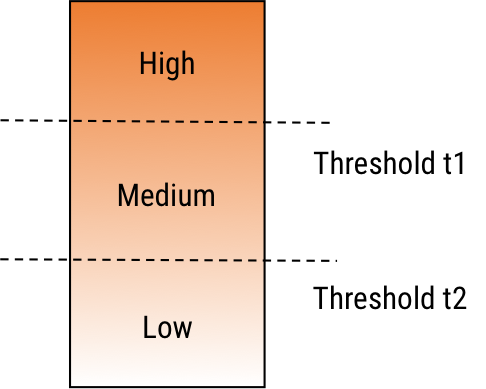
\includegraphics[width=0.3\textwidth]{LevelOfEmotion}
\caption{Level of density of an emotion and thresholds}
\label{fig:levelOfDensity}
\end{figure}

The thresholds are important to detect the abnormal increasing in one particular emotion, yet they are application specific. Firstly, because as their normal behaviour, people tend to post an unequal number of tweets for each emotion, the thresholds can be not the same for different emotions. For instance, happy tweets appear more frequently than angry tweets. Secondly, because of the cultural difference, the content shared on Twitter is very different across different countries and cultures. People in one country might normally post more happy content than people living in a problematic region. Moreover, even among the group of users, emotional content can also vary during different period. For example, people tend to tweet more happy content than usual around Christmas and New Year holiday. Therefore, the choice of the two thresholds for one emotion, such as happy, actually depend on the region and time. In our experiment, we propose an approach to calculate the thresholds using the dataset that is collected in a specific event.

\section{Crowd Model}

The ultimate objective of our crowd monitoring framework is to identify the type of a crowd. Therefore, a crowd model that can describe and differentiate different crowd types is required. From the emergency management point of view, the literature review highlights \citet{Berlonghi1995}'s model as one of the most significant works on crowd types. As mentioned in Chapter \ref{ch:litReview}, \citet{Berlonghi1995} has identified eleven different types of crowd in mass gathering. Each crowd type is described by the movement, participation and behaviour \citep{Zeitz2009}. \citet{Berlonghi1995}'s definition has been widely adopted as the guideline by the emergency bureaus in Australia \citep{EMA1999} and USA \citep{FEMA2005}. Eleven types of crowd are described as below.
\begin{itemize}
\item \textbf{Ambulatory crowd} - is a crowd walking in and out of a venue, to and from parking areas or walking to use restroom or concession facilities.
\item \textbf{Disability/limited movement crowd} - is a crowd of people that in some way are limited or restricted in their movement. Their level or lack of ability to walk, see, hear or speak may require more planning than is provided for all other spectators.
\item \textbf{Cohesive/spectator crowd} is a crowd watching the activities of an event or at the scene of an accident. Its primary character is the fact that people are interested in watching something specific that they came to see.
\item \textbf{Expressive/revellous crowd} - is one involved in some sort of an emotional release which can include cheering, movement in unison, celebrating, dancing, chanting or singing.
\item \textbf{Participatory crowd} - is the crowd of people involved in the actual activities of an event. Sometimes these people may be professional performers or athletes. At other times the people attending the event are participating in an actual sport, such as a marathon. Children may go up onto a stage to perform at the invitation of professional performers.
\item \textbf{Aggressive/hostile crowd} - is one that is becoming verbally aggressive towards or disregarding the instructions of ticket takers, ushers or security personnel. This crowd can get threateningly rowdy and is very open to lawlessness.
\item \textbf{Demonstrator crowd} - is one that is organised to some degree by some established leadership and whose actions may include picketing, marching, chanting or demonstrating at a particular location for a specific purpose.
\item \textbf{Escaping/trampling crowd} - is one that is attempting to escape from danger either of an actual or imagined threat to life. This includes a crowd involved in an organised evacuation procedure and a panic mob pushing and shoving with no order whatsoever.
\item \textbf{Dense/suffocating crowd} - is one in which individual physical movement is rapidly becoming less likely or impossible due to the density of the crowd. People are attempting to move,but they are either swept along with the movement of the crowd or are falling on top of each other. The results of this compression of people are fatalities and serious injuries due to suffocation.
\item \textbf{Rushing/looting crowd} - is one whose principal purpose is to obtain, acquire or steal something. This includes rushing to get the most preferred seats, autographs or actually stealing property. This very often results in fatalities, serious injuries and considerable property damage.
\item \textbf{Violent crowd} - is a crowd that is attacking, terrorising and rioting with complete disregard for laws and the rights of others.
\end{itemize}
However, relying only on the description, it is difficult to make distinct of different crowd types without human observation and judgement on the spot. Therefore, there is a need to introduce attributes or features to the existing model for a systematic approach to perform the classification of crowd type. In this proposal framework, the four basic emotions: anger, fear, happy and sadness are introduced as the features of \citet{Berlonghi1995}'s crowd types. The next section focuses on how the mapping between each crowd type and its associated emotion is constructed.

\section{Emotion - Crowd Type Mapping Model}
In the previous sections, we have discussed the possibility to detect the emotions in a crowd. In our approach, anger, fear, happiness and sadness are used as the four features of a crowd type. This section will explore further into the relationship between each crowd type and each emotion. 

Our mapping is based on several significant studies on human emotion. One of the theory is \citet{Plutchik1980}'s psychoevolutionary theory of emotion which explains emotion as a apart of evolutionary process. According to this theory, the emotional process can be modelled by a sequential model which starts with stimulus events. Based on the interpretation or cognition of these events, humans feel the emotions accordingly. The feeling state of emotion then triggers the overt behaviours or actions to achieve a desired effect. Table \ref{table:sequentialModelOfEmotion} presents the primitive sequential model of emotional process.

\begin{table}
\caption{Sequential model of the emotional process (Taken from \citet{plutchik2001integration})}
\label{table:sequentialModelOfEmotion}
\centering
\begin{tabular}{|p{2.5cm}|p{2.3cm}|p{2.3cm}|p{2.3cm}|p{3.5cm}|}
\hline
\textbf{Stimulus events} & \textbf{Coginition} & \textbf{Emotion} & \textbf{Behaviour} & \textbf{Effect} \\
\hline
Threat & Danger & Fear & Escape & Safety \\
\hline
Obstacle & Enemy & Anger & Attack & Destroy obstacle \\
\hline
Gain of valued object & Possess & Joy & Retain or repeat & Gain resources or new genes \\
\hline
Loss of valued object & Abandonment & Sadness & Cry & Reattach with lost object \\
\hline
Member of a group & Friend & Acceptance (Trust) & Groom & Mutual support \\
\hline
Unpalatable object & Poison & Disgust & Vomit & Eject poison \\
\hline
New territory & Examine & Expectation & Map & Knowledge of territory \\
\hline
Unexpected event & What is it & Surprise & Stop & Gain time to orient \\
\hline
\end{tabular}
\end{table}

In one of his works, \citet{plutchik2001integration} has also summarised the relationship between emotions and their derivatives including their behaviour language, functional language and trait language. The functional language presents the pattern of adaptation to the stimulus event while the behaviour language can describe the actual actions that are derived from a specific emotion. The trait language refers to the personality that is related to that emotion. For example, fear can trigger the escaping action, for the course of protection, and it is caused by timidity. Table \ref{table:derivationOfEmotion} shows the derivation of the eight emotions including fear, anger, happiness and sadness. Although the psychoevolutionary theory is based on the basic emotions and their very primitive stimuli and derivative behaviours, it can still be applied to the modern crowd in our context. A crowd type that we can observe, can be both the stimulus events triggering the emotions or the overt behaviours triggered by the emotions. 

\begin{table}
\caption{Emotions and their derivatives (Taken from \citet{plutchik2001integration})}
\label{table:derivationOfEmotion}
\centering
\begin{tabular}{|p{3cm}|p{3cm}|p{3cm}|p{3cm}|}
\hline
\textbf{Emotion} & \textbf{Behaviour language} & \textbf{Functional language} & \textbf{Trait language} \\
\hline
Fear & Escape & Protection & Timid \\
\hline
Anger & Attack & Destruction & Quarrelsome \\
\hline
Joy & Mate & Reproduction & Sociable \\
\hline
Sadness & Cry & Reattachment & Gloomy \\
\hline
Acceptance (Trust) & Groom & Incorporation & Trusting \\
\hline
Disgust & Vomit & Rejection & Hostile \\
\hline
Expectation & Map & Exploration & Demanding \\
\hline
Surprise & Stop & Orientation & Indecisive \\
\hline
\end{tabular}
\end{table}

Regarding the emotional language, another notable work that plays an important role in our construction of the mapping is from \citet{russell1980circumplex}. In this study, 28 emotional works are placed into a two dimensional space based on their degree of arousal and pleasure (see Figure \ref{fig:emotionSpace}). These affective words include \textit{angry}, \textit{afraid}, \textit{happy} and \textit{sad} which are used to refer the four basic emotions: \textit{anger}, \textit{fear}, \textit{happiness}, \textit{sadness} respectively. From this map, the relative position of a word from the four basic emotions can be observed.

\begin{figure}[htb!] 
\centering    
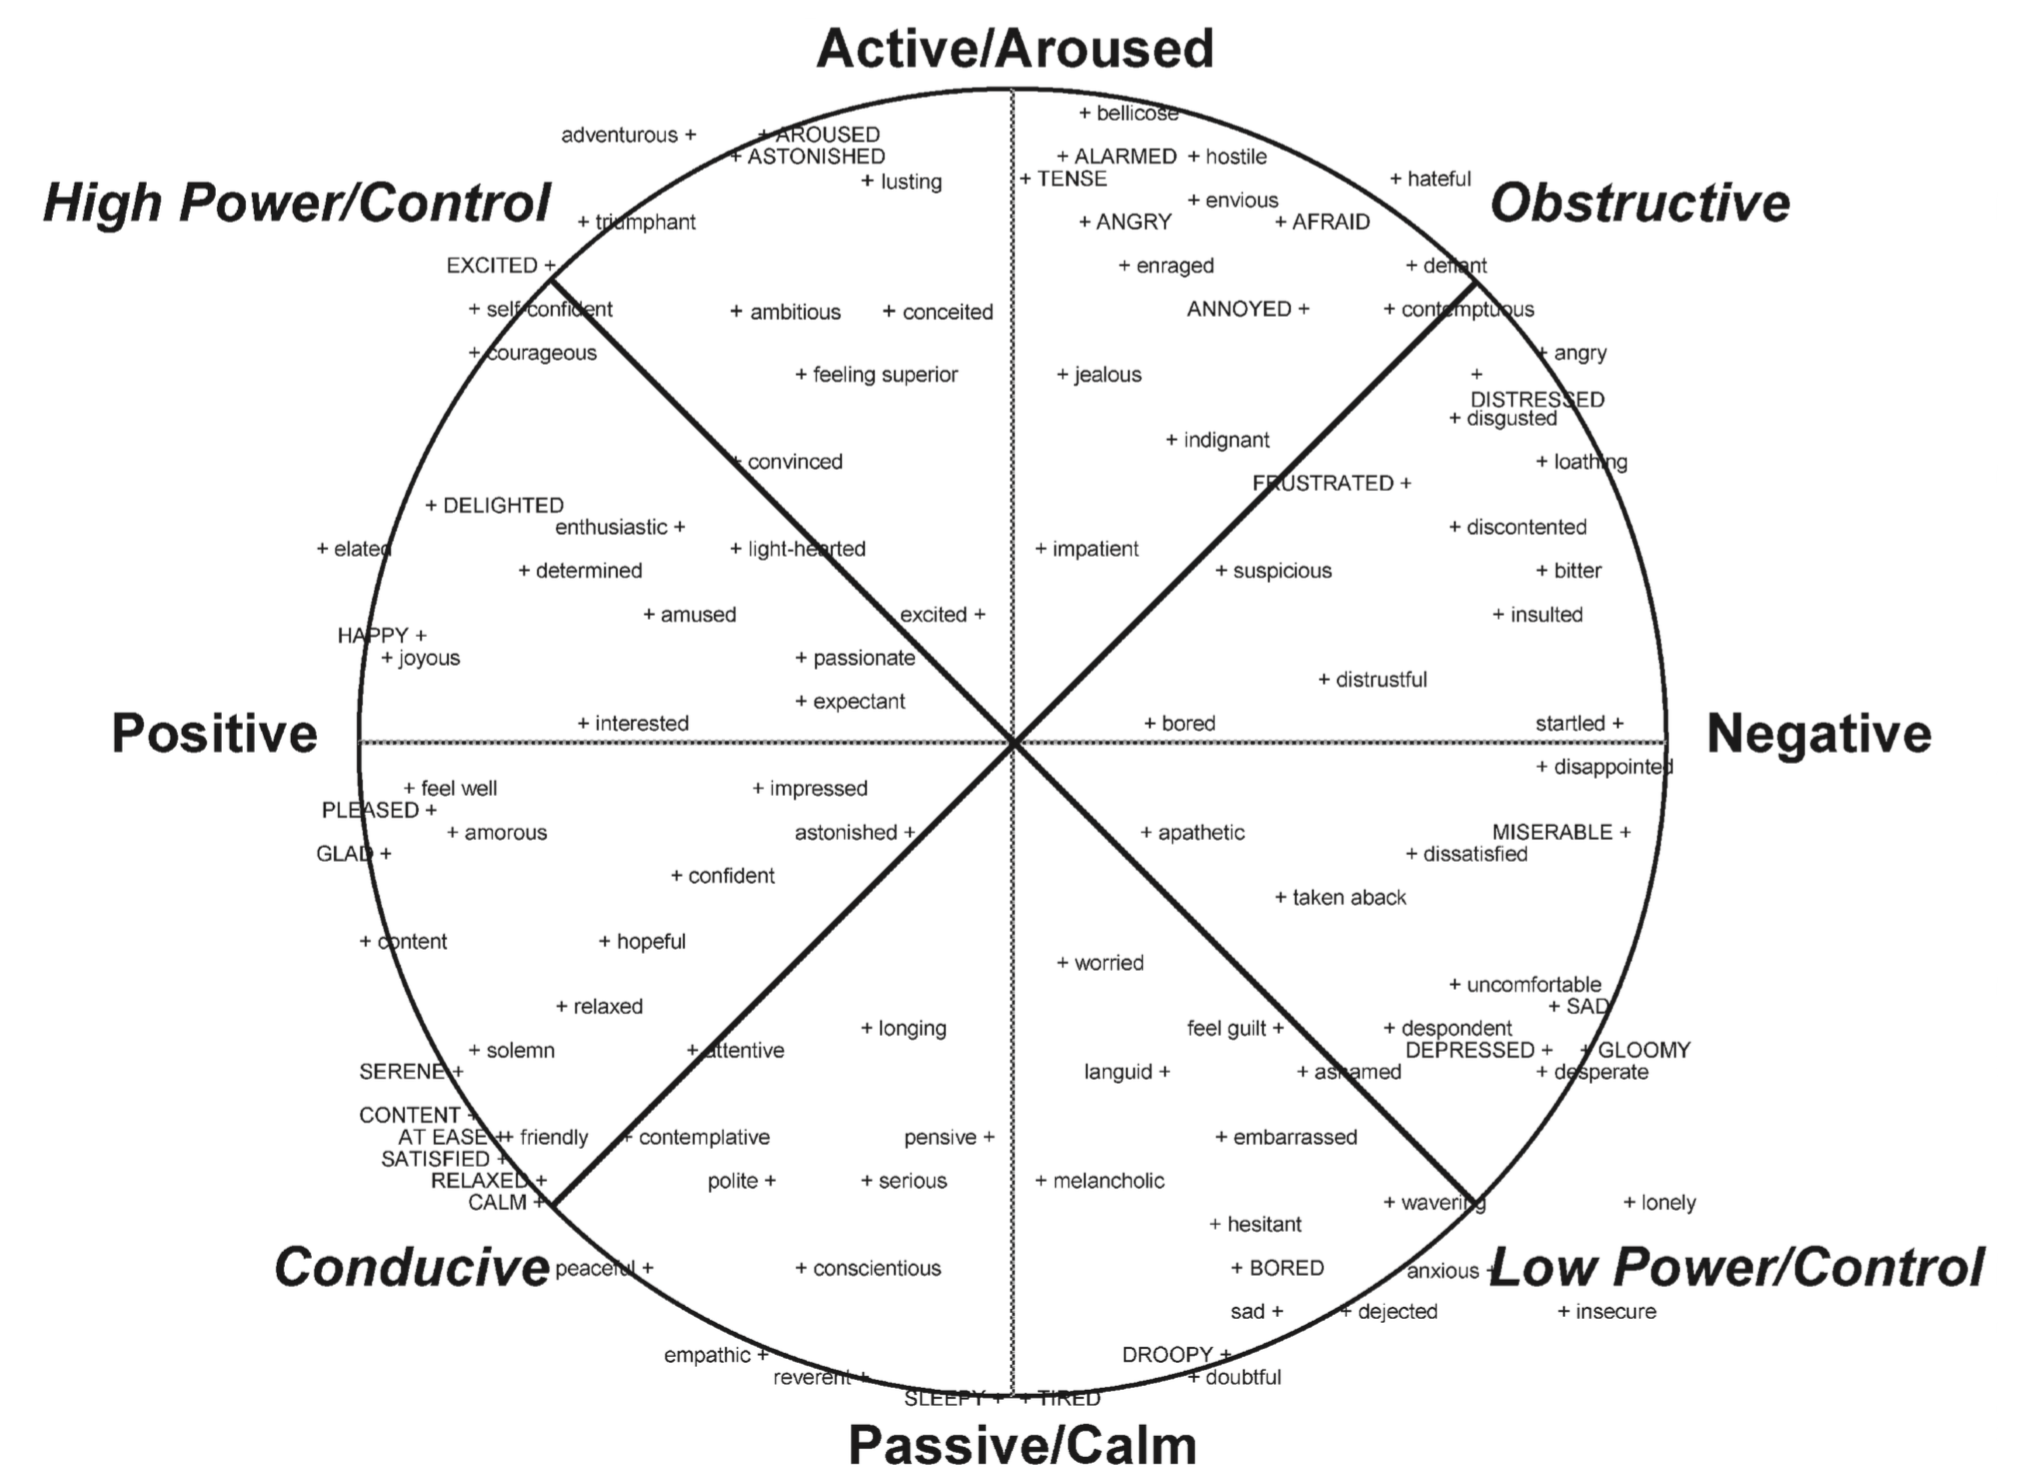
\includegraphics[width=1.0\textwidth]{EmotionSpace}
\caption{Russell's two dimensional map of emotion space (Adapted from \citet{scherer2005emotions})}
\label{fig:emotionSpace}
\end{figure}

In order to construct the emotion - crowd type mapping, a comprehensive understanding of the behaviour of each crowd type is needed. The description of the each crowd type by \citet{Berlonghi1995} is analysed together with the definition of similar crowd types defined by other scholars. The behaviour language and trait language from those descriptions are extracted and referenced to the four emotions: fear, anger, happiness, sadness. The objective of this process is to identify the dominant emotions in each crowd type. 

\begin{itemize}
\item \textbf{Ambulatory crowd} - is characterised by the action walking and the calmness \citep{Zeitz2009}. According to \citet{russell1980circumplex}'s emotion space, \textit{calm} is located in a completely opposite region with \textit{angry} and \textit{afraid}. Although both \textit{calm} and \textit{sad} have negative level of arousal, the former has a positive degree of pleasure while the latter does not. Therefore, none of the four emotions are dominating in this crowd type.
\item \textbf{Disablity/Limited movement crowd} - is described by the immobility of the crowd. Similarly to the ambulatory crowd, this characteristic does not suggest any significant emotion. Hence, no emotion is considered to be the dominant emotion in this crowd type.
\item \textbf{Cohesive/Spectator} - is described by the activity watching a specific event and the fact that people have the interest in watching the event. Similarly, they do not signal the dominant occurrence of any emotion.
\item \textbf{Expressive/Revellous crowd} - is characterised by the emotional release. According to the Webster's Revised Unabridged Dictionary \footnote{http://www.thefreedictionary.com/revelous}, the word \textit{revelous} originates from ``revel'' which means ``to take great pleasure or delight'' \footnote{http://www.thefreedictionary.com/reveling}. \textit{Delighted} lies in a high level of arousal with a positive pleasure in the \citet{russell1980circumplex}'s emotion space (Figure \ref{fig:emotionSpace}), which is close to \textit{happy}. Therefore, it can be inferred that this crowd type has a high intensity of \textit{happiness} as the dominant emotion.
\item \textbf{Participatory crowd} - is described by the action participating in a specific event. Although, the description does not suggest any clue on the emotional state of the participants, one example for a participatory crowd is people taking part in an actual sport event. Regarding sport psychology, studies show that sensation seeking and arousal seeking motivate the participations in sports, especially risk involved sports \citep{rowland1986sensation}. This indicates a positive level of arousal that can be observed from a participatory crowd, thus suggesting \textit{happiness} as the dominating emotion as well. Compared to expressive crowd, the intensity of \textit{happiness} can be lower.
\item \textbf{Aggressive/Hostile crowd} - is described by the verbal aggressiveness and disregard for instruction. \textit{Aggressiveness} is aroused by \textit{anger}. The \textit{aggressiveness} is limited by verbal expression, which hints that the intensity of \textit{anger} is at medium level.
\item \textbf{Demonstrator} - includes such actions as picketing, marching, protesting. According to Lofland's typology of spontaneous collective behaviours \citep{Kornblum2011}, such crowds are classified into \textit{hostile} crowd aroused by \textit{anger}. This crowd type is described to have some degree of organisation and leadership, which suggests the level of \textit{aggressiveness} is not intensive. Therefore, a low level of \textit{anger} can be considered to be the dominant emotion in this crowd type.
\item \textbf{Escaping/Trampling crowd} - is described by the escaping action from a danger or a threat. This \textit{escaping} behaviour is triggered by \textit{fear} according to Plutchik's evolutionary theory. Loftland's typology also classifies such crowd under the fearful crowd \cite{Kornblum2011}. Hence, the dominating emotion can be identified in this crowd type is clearly a high intensity of \textit{fear}.
\item \textbf{Dense/Suffocating crowd} - is characterised by the extremely high density and inability of movement in the crowd. Recent research on brain claims that suffocation might cause fear as the experiments with mice shows that inhaled carbon dioxide reduces brain pH and evokes fear behaviour \citep{ziemann2009amygdala}.
\item \textbf{Rushing/Looting crowd} - is described by the desire to acquire something. Studying the looting behaviour in London riot in 2011, \citet{ray2014shame} suggests the shame theory of violence which might has relevance in accounting for the violent disturbance. \textit{Shame} falls into the region with low arousal and negative pleasure together with the basic emotion \textit{sad}, which indicates the closeness of the two affective words. On the other hand, violence is aroused by \textit{anger}, hence a mixture of \textit{anger} and \textit{sadness} can be considered the dominating emotions in a looting crowd.
\item \textbf{Violent crowd} - is described by the attacking, terrorising and rioting action with the complete disregard for laws and other people. Attacking is a typical behaviour triggered by \textit{anger}. This crowd type has a high level of \textit{anger}.
\end{itemize}

As we can notice from above analysis, five distinct groups of crowd types can be identified by the similarity in the dominating emotions. Although it might be challenging to distinguish different crowd types in the same group using the emotional states as the criteria, it is possible to extend the framework and incorporate additional information sources and analysis to provide more low level and high level context data used in classification, for example accelerometer and activity recognition. However, obtaining data from the sensors in participants' mobile phones requires installing software on those devices, which might cause he hesitance to share information or privacy concern. Therefore, our proposed framework only focuses on the social media analysis, which is more feasible in favour of deployment.

\begin{itemize}
\item The first group consists of ambulatory, disability/limited movement and cohesive/spectator crowd, which suggest no dominant emotion. From the emergency management point of view, those three types do not pose potential danger. Therefore, in our crowd monitoring framework, the three crowd types will be grouped and monitored as a same type. As mentioned earlier, if data from accelerometer on participants' mobile devices can be acquired, the activities of participants in the crowd can be inferred using activity recognition technique. In term of the type of activity, an ambulatory crowd involves mostly walking, while a crowd of spectators or limited movement crowd will be more stationary with such actions as sitting or standing.

\item The second group is characterised by \textit{happiness}. Expressive/revellous and participatory crowd belong to this group. The difference between an expressive and a participatory crowd is the level of happiness which is high in the former crowd and medium in the latter crowd type. Similarly, to further distinguish between these two crowd types, using accelerometer and activity recognition to infer the activities of the participants might be a possible solution. If the activities involve lots of movement such as running and walking, the crowd can be identified as a participatory crowd.

\item The third group is aroused by \textit{anger} and includes demonstrator, aggressive/hostile and violent crowd with the increasing level of anger. Activity recognition can also be used to give additional knowledge. A violent crowd involves activities that have a higher level of motion such as running and walking, while a demonstrator crowd might have a slower pace of movement.

\item The fourth group is motivated by \textit{fear} consisting of escaping/trampling and dense/suffocating crowd. Because a dense/suffocating crowd is characterised by the high density and the inability to move, this crowd type can be identified with most people standing by activity recognition.

\item The fifth group is rushing/looting crowd which has both \textit{anger} and \textit{sadness} as the dominant emotions.
\end{itemize}

\begin{table}
\caption{Mapping between crowd types and emotions}
\label{table:mappingEmotionCrowdType}
\begin{tabular}{|p{1.4cm}|p{5.1cm}|p{1.6cm}|p{1.5cm}|p{1.9cm}|p{1.6cm}|}
\hline
\textbf{Group} & \textbf{Crowd type} & \textbf{Anger} & \textbf{Fear} & \textbf{Happiness} & \textbf{Sadness} \\
\hline
\multirow{3}{\linewidth}{Group 1} & Ambulatory & & & & \\
\cline{2-6}
& Disability / Limited movement & & & & \\
\cline{2-6}
& Cohesive / Spectator & & & & \\
\hline
\multirow{2}{\linewidth}{Group 2} & Expressive / Revellous & & & high & \\
\cline{2-6}
& Participatory & & & medium & \\
\hline
\multirow{3}{\linewidth}{Group 3} & Aggressive / Hostile & medium & & & \\
\cline{2-6}
& Demonstrator & low &  &  & \\
\cline{2-6}
& Violent & high & & & \\
\hline
\multirow{2}{\linewidth}{Group 4} & Escaping / Trampling & & high & & \\
\cline{2-6}
& Dense / Suffocating & & high & & \\
\hline
Group 5 & Rushing / Looting & medium & & & medium \\
\hline
\end{tabular}
\end{table}

\section{Rule Based Reasoning}

\subsection{Rule Repository}
The Rule Repository contains the rules to identify a crowd type from the inferred emotional state of the crowd.

\begin{equation}
	
\end{equation}

\subsection{Rule Base Reasoning}

\section{Conclusion}